\usetikzlibrary{plotmarks}

\begin{figure}[htbp]
\centering
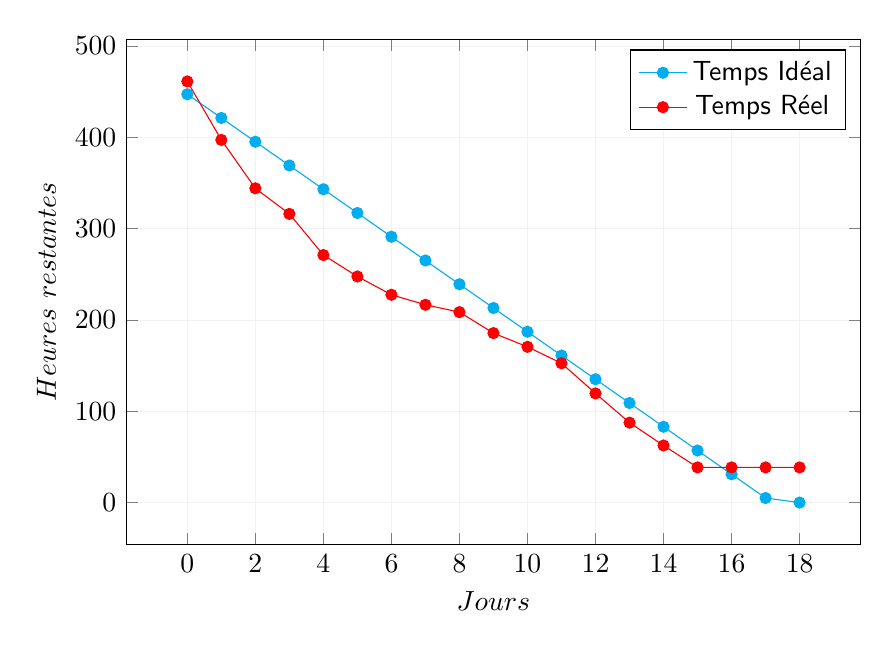
\begin{tikzpicture}[y=.2cm, x=.7cm,font=\sffamily]
\begin{axis}[
xlabel=$Jours$,
ylabel=$Heures\ restantes$,
grid=both,
grid style={line width=.1pt, draw=gray!10},
width=0.9\textwidth,
height=8cm,
%major grid style={line width=.2pt,draw=gray!50},
]
      \addplot[mark=*,cyan] plot coordinates {%

              (0, 447)
              (1, 421)
              (2, 395)
              (3, 369)
              (4, 343)
              (5, 317)
              (6, 291)
              (7, 265)
              (8, 239)
              (9, 213)
              (10, 187)
              (11, 161)
              (12, 135)
              (13, 109)
              (14, 83)
              (15, 57)
              (16, 31)
              (17, 5)
              (18, 0)
    };
    \addlegendentry{Temps Idéal}

    \addplot[mark=*,red] plot coordinates {%
        (0, 461)
        (1, 397)
        (2, 344)
        (3, 316)
        (4, 271)
        (5, 247.5)
        (6, 227.5)
        (7, 216.5)
        (8, 208.5)
        (9, 185.5)
        (10, 170.5)
        (11, 152.5)
        (12, 119.5)
        (13, 87.5)
        (14, 62.5)
        (15, 38.5)
        (16, 38.5)
        (17, 38.5)
        (18, 38.5)
    };
    \addlegendentry{Temps Réel}
\end{axis}
\end{tikzpicture}
\caption{Graphique d'avancement - Itération 3}
\label{fig:sprint3-burndown}
\end{figure}
